\subsection{Пропорциональная селекция}\label{SetOfOperatorsAlgorithms:ProportionalSelection}

Идентификатор: \textbf{ProportionalSelection}.

Вероятность выбора элемента пропорциональна значению пригодности индивида. Данный вид селекции может работать только с неотрицательными значениями пригодности.

Пропорциональная селекция определяется формулой:

\begin{equation}
\label{SetOfOperatorsAlgorithms:eq:ProportionalSelection}
Selection\left( Population, Fitness, DataOfSel\right) = Random\left( \left\lbrace\bar{x}^i | p^i \right\rbrace \right),
\end{equation}
\begin{equation}
p^i=\left\lbrace \begin{aligned}
\dfrac{f_{fit}\left( \bar{x}^i\right) }{\sum_{j=1}^N{f_{fit}\left( \bar{x}^j\right)}},&\text { если }  \exists f_{fit}\left( \bar{x}^k\right)\neq 0 \left( k=\overline{1,N} \right); \\ \dfrac{1}{N} ,&\text { иначе}.
\end{aligned}\right.
\end{equation}

где $ \bar{x}^i \in Population, i=\overline{1,N} $.

Как видим, формула определения вероятности выбора индивида имеет составной вид. Второе условие предназначено для маловероятного случая, когда в популяции все индивиды будут иметь пригодность равную нулю.

\textbf{Пример.} Пусть $ Fitness=\left\lbrace 0,5; 0,2; 0,1; 0,6; 0,2; 0,4\right\rbrace $. Тогда вероятности выбора индивидов равны:
\begin{flalign*}
p_1&=\frac{0,5}{0,5 + 0,2 + 0,1 + 0,6 + 0,2 + 0,4}=0,25;\\
p_2&=\frac{0,2}{0,5 + 0,2 + 0,1 + 0,6 + 0,2 + 0,4}=0,1;\\
p_3&=\frac{0,1}{0,5 + 0,2 + 0,1 + 0,6 + 0,2 + 0,4}=0,05;\\
p_4&=\frac{0,6}{0,5 + 0,2 + 0,1 + 0,6 + 0,2 + 0,4}=0,3;\\
p_5&=\frac{0,2}{0,5 + 0,2 + 0,1 + 0,6 + 0,2 + 0,4}=0,1;\\
p_6&=\frac{0,4}{0,5 + 0,2 + 0,1 + 0,6 + 0,2 + 0,4}=0,2.
\end{flalign*}

\begin{figure} [H] 
  \center
  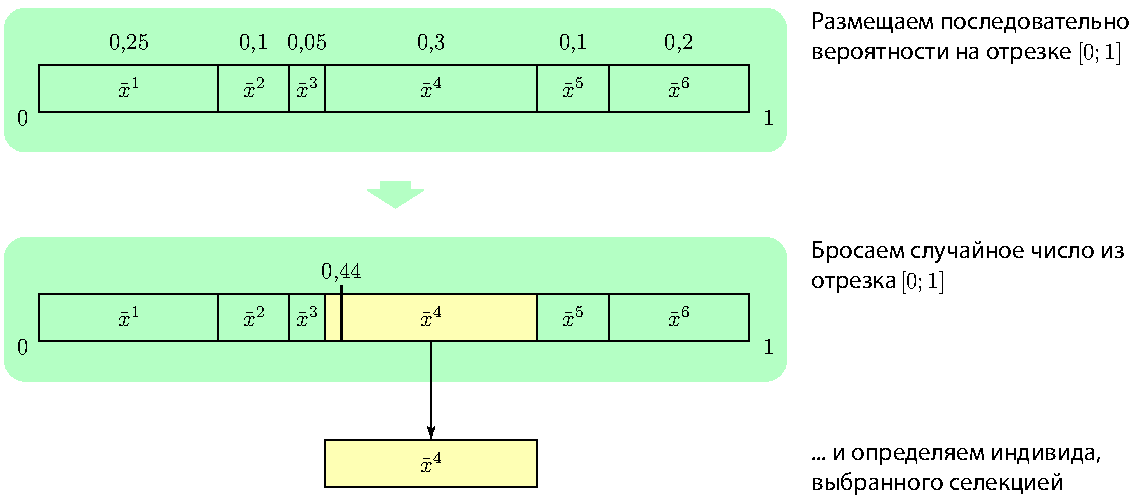
\includegraphics [scale=0.7] {ProportionalSelection}
  \caption{Механизм работы пропорциональной селекции} 
  \label{SetOfOperatorsAlgorithms:img:ProportionalSelection}  
\end{figure}

$ DataOfSel $ также не содержит каких-либо параметров относительно данного типа селекции.

Нет ограничений на множество задач оптимизации, которые может решать алгоритм оптимизации с данной селекцией. 

В библиотеке \textbf{HarrixMathLibrary} данная селекция реализуется через функции \textbf{HML\_ProportionalSelection}, \textbf{HML\_ProportionalSelectionV2} и \textbf{HML\_ProportionalSelectionV3}:

\href{https://github.com/Harrix/HarrixMathLibrary}{https://github.com/Harrix/HarrixMathLibrary}